%; whizzy section -pdf xpdf -latex ./whizzypdfptex.sh
% latex beamer presentation.
% platex, latex-beamer $B$G%3%s%Q%$%k$9$k$3$H$rA[Dj!%(B 

%     Tokyo Debian Meeting resources
%     Copyright (C) 2008 Junichi Uekawa

%     This program is free software; you can redistribute it and/or modify
%     it under the terms of the GNU General Public License as published by
%     the Free Software Foundation; either version 2 of the License, or
%     (at your option) any later version.

%     This program is distributed in the hope that it will be useful,
%     but WITHOUT ANY WARRANTY; without even the implied warranty of
%     MERCHANTABILITY or FITNESS FOR A PARTICULAR PURPOSE.  See the
%     GNU General Public License for more details.

%     You should have received a copy of the GNU General Public License
%     along with this program; if not, write to the Free Software
%     Foundation, Inc., 51 Franklin St, Fifth Floor, Boston, MA  02110-1301 USA

\documentclass[cjk,dvipdfm,12pt]{beamer}
\usetheme{Tokyo}
\usepackage{monthlypresentation}

%  preview (shell-command (concat "evince " (replace-regexp-in-string "tex$" "pdf"(buffer-file-name)) "&"))
%  presentation (shell-command (concat "xpdf -fullscreen " (replace-regexp-in-string "tex$" "pdf"(buffer-file-name)) "&"))

%http://www.naney.org/diki/dk/hyperref.html
%$BF|K\8l(BEUC$B7O4D6-$N;~(B
\AtBeginDvi{\special{pdf:tounicode EUC-UCS2}}
%$B%7%U%H(BJIS$B7O4D6-$N;~(B
%\AtBeginDvi{\special{pdf:tounicode 90ms-RKSJ-UCS2}}

\title{Debian Project and the Development Process, and how to co-work
with it.}
\subtitle{Cooperating with a large open source community}
\author{$B>e@n(B $B=c0l(B Junichi Uekawa\\dancer@debian.org\\IRC nick: dancerj}
\date{eeePC Developers' Conference 9 April 2008}
\logo{
\includegraphics[width=8cm]{../base-image/openlogo-light.eps}}

\begin{document}

\frame{\titlepage{}}

% draft framework of talk.

\begin{frame}{$B>e@n=c0l(B}
\begin{itemize}
 \item 2000$BG/(B- Debian Developer
 \item 2006$BG/(B- Debian JP Project $B2qD9(B
 \item Debian $B$N$$$/$D$+$N%D!<%k!"(B
       pbuilder, dpatch, cowdancer, dsh $BEy$N4IM}(B
\end{itemize}
\end{frame}

\begin{frame}{Junichi Uekawa}
\begin{itemize}
 \item Debian Developer since 2000
 \item Leading Debian JP Project since 2006
 \item Developer and maintainer of several Debian tools, such
       as pbuilder, dpatch, cowdancer, dsh, etc.
\end{itemize}
\end{frame}

\begin{frame}{What is Debian Project}
 \begin{itemize}%[<+->]
  \item 1 social contract, policy
  \item 11\footnote{etch official architectures} architectures 
  \item 215\footnote{as of 8 May 2008} mailing lists
  \item 1075\footnote{developers who can vote as of March 2008 DPL election}
	maintainers 
	\footnote{2093 if including 755 with packages, 
	1338 sponsored people, according to \url{http://io.debian.net/~tar/bugstats/}}
  \item 10223\footnote{etch official source packages count, sid has 13574 as
	of 8 May 2008} packages
  \item All for Free Software.
 \end{itemize}
\end{frame}

\begin{frame}{What is Debian Distribution}
\begin{itemize}
 \item Debian GNU/Linux (i386) and Debian GNU/Linux (amd64) being the
       most used product.
 \item Not specific focus on Desktop or laptop or Server or embedded; tries to serve all.
 \item many architectures
 \item many kernels: Linux, kFreeBSD, Hurd....
 \item Focus on DFSG, based on policy
\end{itemize}
\end{frame}


\begin{frame}{Debian Communication framework }

Developers are distributed all around the world:

 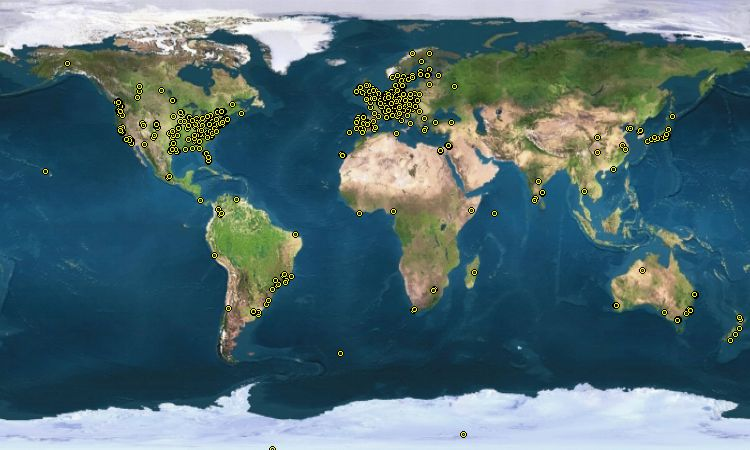
\includegraphics[width=1\hsize]{image200805/developers-map.jpeg} 

\end{frame}

\begin{frame}{Debian Communication framework }

\begin{itemize}
 \item  We are all different

 \item  We need a distributed process.
\end{itemize}

\end{frame}

\begin{frame}{What is Debian Distribution}
\begin{itemize}
 \item DFSG: Debian Free Software Guidelines
 \item Debian Policy: minimal guidelines on how packages should behave
 \item specific policies: smaller policies govern more minor parts of
       packaging; rules evolve. c.f. emacs policy, ruby policy, etc.
\end{itemize}
\end{frame}

\begin{frame}{Debian Communication framework}
 \begin{itemize}
  \item mailing lists and archives (lists.debian.org)
  \item IRC network (irc.debian.org)
  \item BTS (bugs.debian.org)
  \item Wiki (wiki.debian.org)
  \item svn, Git, ... (alioth.debian.org, svn.debian.org,
	git.debian.org, ...)
 \end{itemize}

BTS (and the mailing lists) and supporting framework support the community

\end{frame}

\begin{frame}{Debian Development Process}

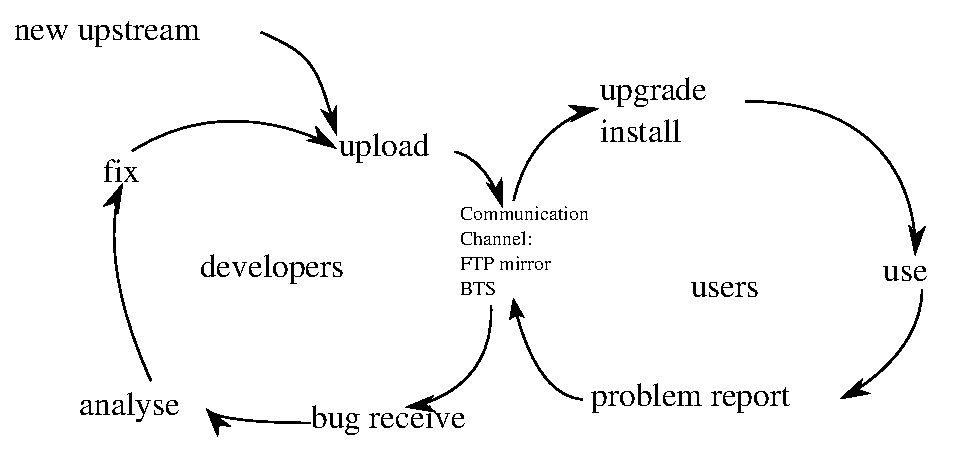
\includegraphics[width=1\hsize]{image200805/develcycle.eps} 

All processes are package-centric

\end{frame}

\begin{frame}{User Process: Install / Upgrade}
 \begin{itemize}
  \item new package: 
	user searches via apt-cache search, or finds out about package,
	and installs it via apt-get install / aptitude install / ...
  \item upgraded package:
	user upgrades package through 
	apt-get  / aptitude.	
 \end{itemize}
\end{frame}

\begin{frame}{User Process: the analysis workflow}
\begin{minipage}{0.40\hsize}
 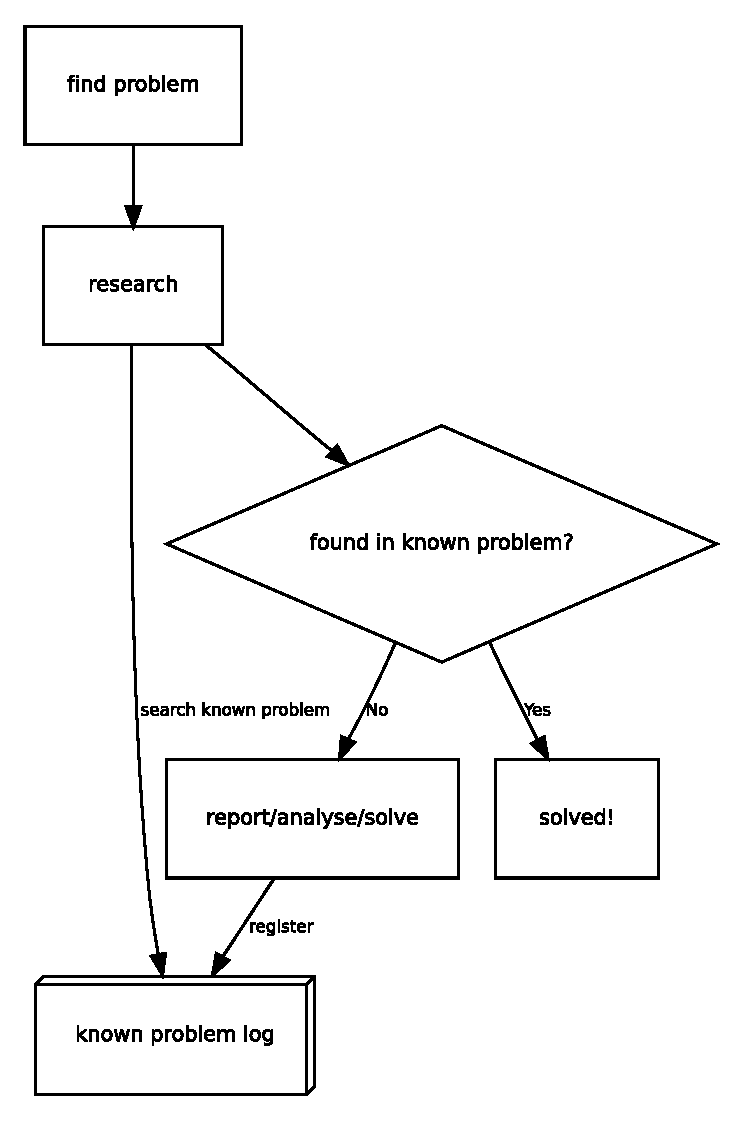
\includegraphics[width=1\hsize]{image200805/problemcycle-en.eps}
\end{minipage}
\begin{minipage}{0.5\hsize}
 \begin{itemize}
  \item User uses the package
  \item User finds the problem
  \item User reports the problem
  \item Optionally: User fixes the problem
 \end{itemize}
\end{minipage}
\end{frame}

\begin{frame}{Tool: debconf}

Common interface to ask users questions.

 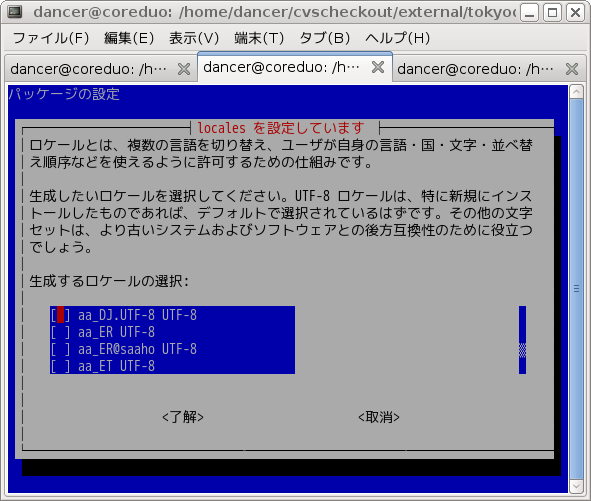
\includegraphics[width=0.5\hsize]{image200805/debconf-text.png}
 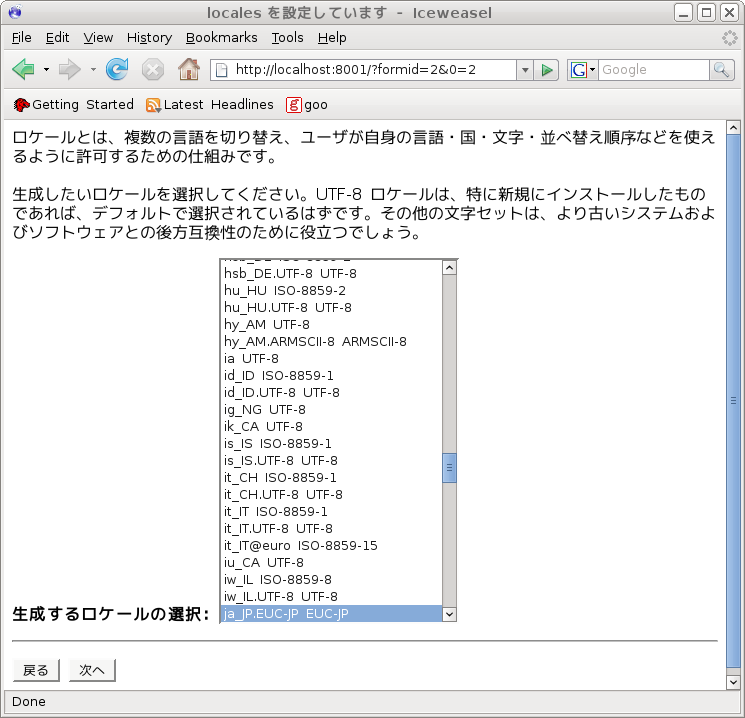
\includegraphics[width=0.5\hsize]{image200805/debconf-locales.png}

\end{frame}

\begin{frame}[containsverbatim]{Tool: apt-listbugs}
\begin{commandline}
dancer@debian:~$ sudo apt-get install dpkg apt
 .
 .
 .
Found/Fixed $B>pJs$r2r@O$7$F$$$^$9(B... $B40N;(B
$B%P%0(B serious/apt (0.7.11 -> 0.7.12) <done>
 #476696 - cdebootstrap should install recommends (debian-archive-keyring/2008.04.16+nmu1 $B$G=$@5(B)
   $B0J2<$N%P%0$HE}9g$5$l$F$$$^$9(B: 476532 476689
$B%P%0(B grave/apt (0.7.11 -> 0.7.12) <pending>
 #474947 - MMap, again; and won't be denied this time
$B%P%0(B serious/apt (0.7.11 -> 0.7.12) <pending>
 #475530 - Internal Error, Could not perform immediate configuration (2) on tzdata
   $B0J2<$N%P%0$HE}9g$5$l$F$$$^$9(B: 464559 466027 466695 467059
$BMWLs(B:
 apt(3 $B8D(B)
$B$3$l$i$N%Q%C%1!<%8$N%$%s%9%H!<%k!&99?7$r7QB3$7$F$h$m$7$$$G$9$+(B? [Y/n/?/...]  
\end{commandline}
\end{frame}

\begin{frame}[containsverbatim]{Tool: apt-listbugs}

Gives the option of not installing a buggy package

\begin{commandline}
dancer@debian:~$ sudo apt-get install dpkg apt
 .
 .
 .
serious bugs of apt (0.7.11 -> 0.7.12) <done>
 #476696 - cdebootstrap should install recommends (Fixed: debian-archive-keyring/2008.04.16+nmu1)
   Merged with: 476532 476689
grave bugs of apt (0.7.11 -> 0.7.12) <pending>
 #474947 - MMap, again; and won't be denied this time
serious bugs of apt (0.7.11 -> 0.7.12) <pending>
 #475530 - Internal Error, Could not perform immediate configuration (2) on tzdata
   Merged with: 464559 466027 466695 467059
Summary:
 apt(3 bugs)
Are you sure you want to install/upgrade the above packages? [Y/n/?/...]  
\end{commandline}
\end{frame}

\section{apt-listchanges 1/2}

\begin{frame}{Tool: apt-listchanges 1/2}
\begin{minipage}{0.49\hsize}
 
 list changelog entries before install.

 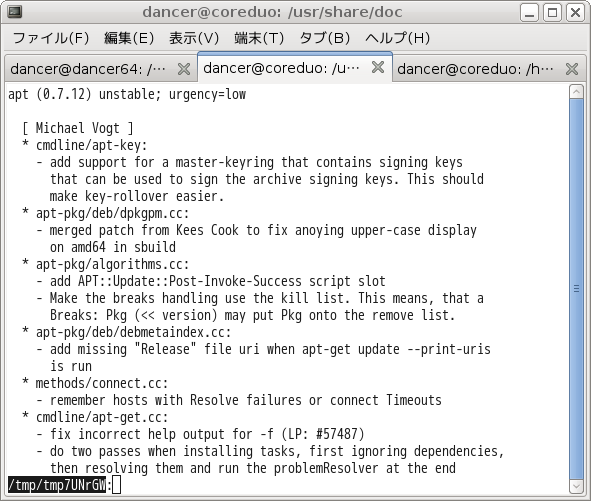
\includegraphics[width=1\hsize]{image200805/apt-listchanges.png}
\end{minipage}

\end{frame}

\begin{frame}[containsverbatim]{Tool: apt-listchanges 2/2}
 \begin{minipage}{0.49\hsize}

 \begin{commandline}
  dpkg-reconfigure apt-listchanges
 \end{commandline} 
 to make apt-listchanges to ask before installing

 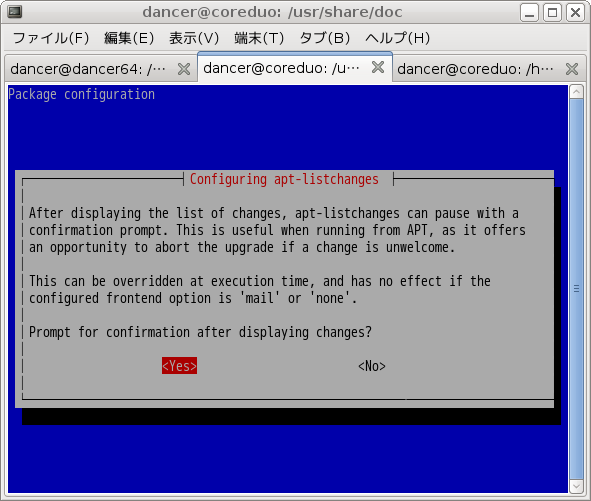
\includegraphics[width=1\hsize]{image200805/apt-listchanges-qa.png}
 \end{minipage}
\end{frame}

\begin{frame}{User Process: using package}
\begin{itemize}
 \item find documentation through 'dpkg -L '.
       \url{/usr/share/doc/PACKAGE/README.Debian}, manpage(1), etc.
 \item read Debian Policy. 
       \url{/usr/share/doc/debian-policy/policy.txt.gz}
\end{itemize}
\end{frame}

\begin{frame}{User Process: Problem Report 1/2}
\begin{itemize}
 \item Sending patches.
 \item Sending reproducible problem.
 \item Sending vague feature requests.
\end{itemize}

What do you want to do today?
\end{frame}

\begin{frame}{User Process: Problem Report 2/2}
Tools to use 
\begin{itemize}
 \item gdb, strace, valgrind, oprofile, etc ... 
 \item \url{http://bugs.debian.org/}
\end{itemize} 
\end{frame}

\begin{frame}{Tool: Bugs.debian.org interface}
Tools to use 
\begin{itemize}
 \item Mail interface.
 \item Web interface.
 \item GUI tools.
\end{itemize} 
\end{frame}

\begin{frame}[containsverbatim]{Tool: Bugs.debian.org interface: Mail}
\begin{itemize}
 \item The BTS commands work by e-mail (SMTP).
 \item Reading BTS is done via HTTP.
\end{itemize}
\begin{commandline}
To: submit@bugs.debian.org
Subject: Bug#429247: refit new upstream version
From: Junichi Uekawa <dancer@netfort.gr.jp>
Message-ID: <87odjgatfz.dancerj%dancer@netfort.gr.jp>

Package: refit
Version: 0.7

0.10 is released upstream, and is probably required for newer
hardware. However, gnu-efi in Debian currrently is too old to build
it.
\end{commandline}
\end{frame}

\begin{frame}[containsverbatim]{Tool: Bugs.debian.org interface: Mail/control}

Bug metadata can be controlled

\begin{commandline}
To: Junichi Uekawa <dancer@netfort.gr.jp>, 474343@bugs.debian.org
Cc: Debian Bug Tracking System <control@bugs.debian.org>
Subject: Re: Bug#474343: grub: update-grub ends with exit code 139
From: Junichi Uekawa <dancer@netfort.gr.jp>
Message-ID: <87d4p31zln.dancerj%dancer@netfort.gr.jp>


reassign 474343 grub-common
severity serious
thanks

grub-probe segfaults on my system.
\end{commandline}
\end{frame}

\begin{frame}[containsverbatim]{Tool: Bugs.debian.org interface: Mail/follow-up}

Bug information is added to mail address

\begin{commandline}
To: Robert Millan <rmh@aybabtu.com>
Cc: Junichi Uekawa <dancer@netfort.gr.jp>, 474343@bugs.debian.org
Subject: Re: Bug#474343: grub: update-grub ends with exit code 139
From: Junichi Uekawa <dancer@netfort.gr.jp>
Message-ID: <87lk3iypx8.dancerj%dancer@netfort.gr.jp>

 .
 .
 .

> Please try also this one (separately) if you can.  It's supposed to
> improve robustness in case similar problems arise.

This also works fine.
\end{commandline}
\end{frame}

\begin{frame}{Tool: Bugs.debian.org interface: Web}

\url{http://bugs.debian.org/474343}

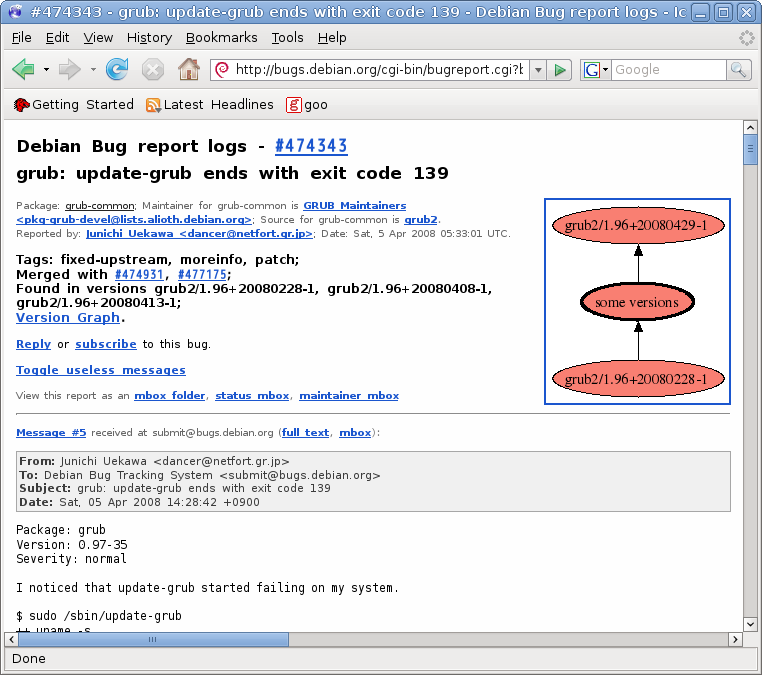
\includegraphics[width=0.6\hsize]{image200805/btsweb.png}
\end{frame}

\begin{frame}{Tool: Bugs.debian.org interface: TUI}
reportbug

 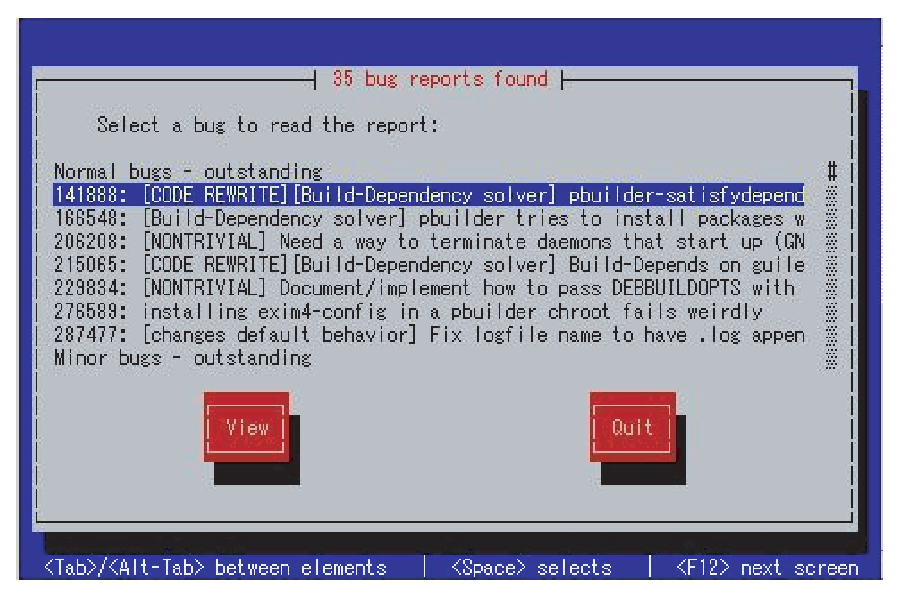
\includegraphics[width=1\hsize]{../2005-resume/image200508/reportbug.eps}
\end{frame}

\begin{frame}{Tool: Bugs.debian.org interface: GUI}

reportbug-ng

 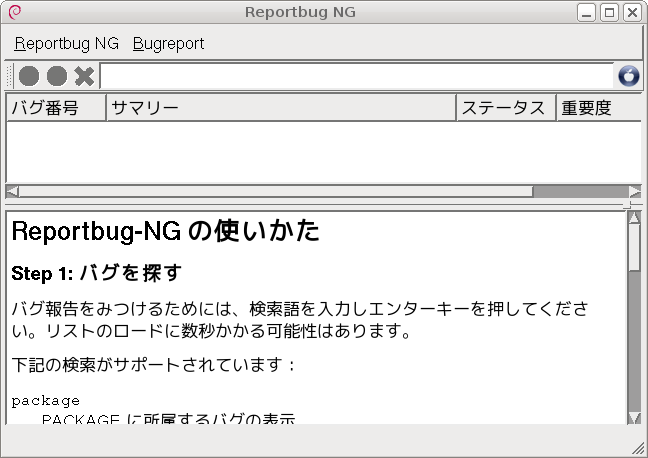
\includegraphics[width=1\hsize]{image200805/reportbug-ng.png}
\end{frame}

\begin{frame}{Debian Development Process}

 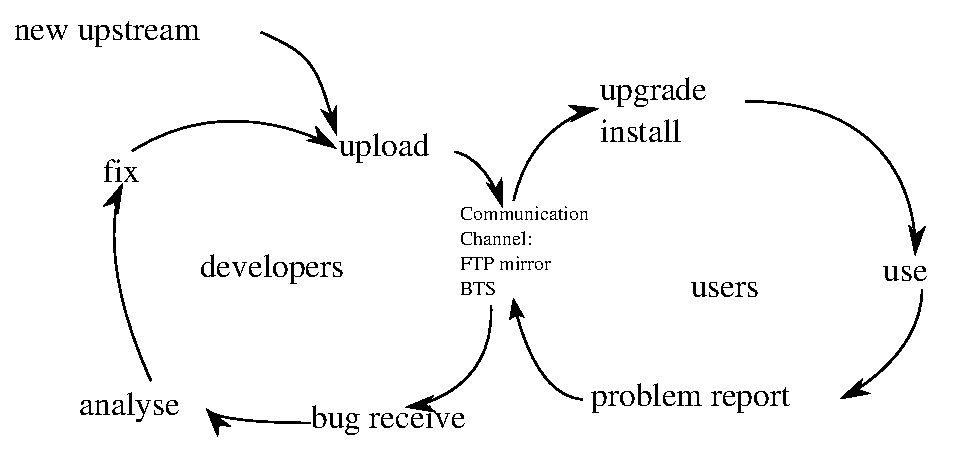
\includegraphics[width=1\hsize]{image200805/develcycle.eps} 

\end{frame}

\begin{frame}{Developer Process: introduction}

 \includegraphics[width=0.4\hsize]{../2007-resume/image200705/develcycle.eps}
\end{frame}

\begin{frame}{Developer Process: upload}
 \begin{itemize}
  \item new package 
  \item new upstream
  \item bug handling:
	bug is closed by fixed package version, or is a non-bug.
  \item package upload is handled twice daily
 \end{itemize}
\end{frame}

\begin{frame}{Developer Process: upload: testing}

 % FIXME too much text
\begin{minipage}{0.5\hsize}
  \begin{itemize}
   \item packages are uploaded to 'unstable', updated twice a day
   \item packages are used by users, and effectively do integration testing.
   \item users will claim Release-Critical-bug
   \item A week of non-bug life == worthy of being used by 'testing'
	 users, and 'testing' is to be the next 'stable' (in two years).
 \end{itemize}
\end{minipage}
\begin{minipage}{0.4\hsize}
 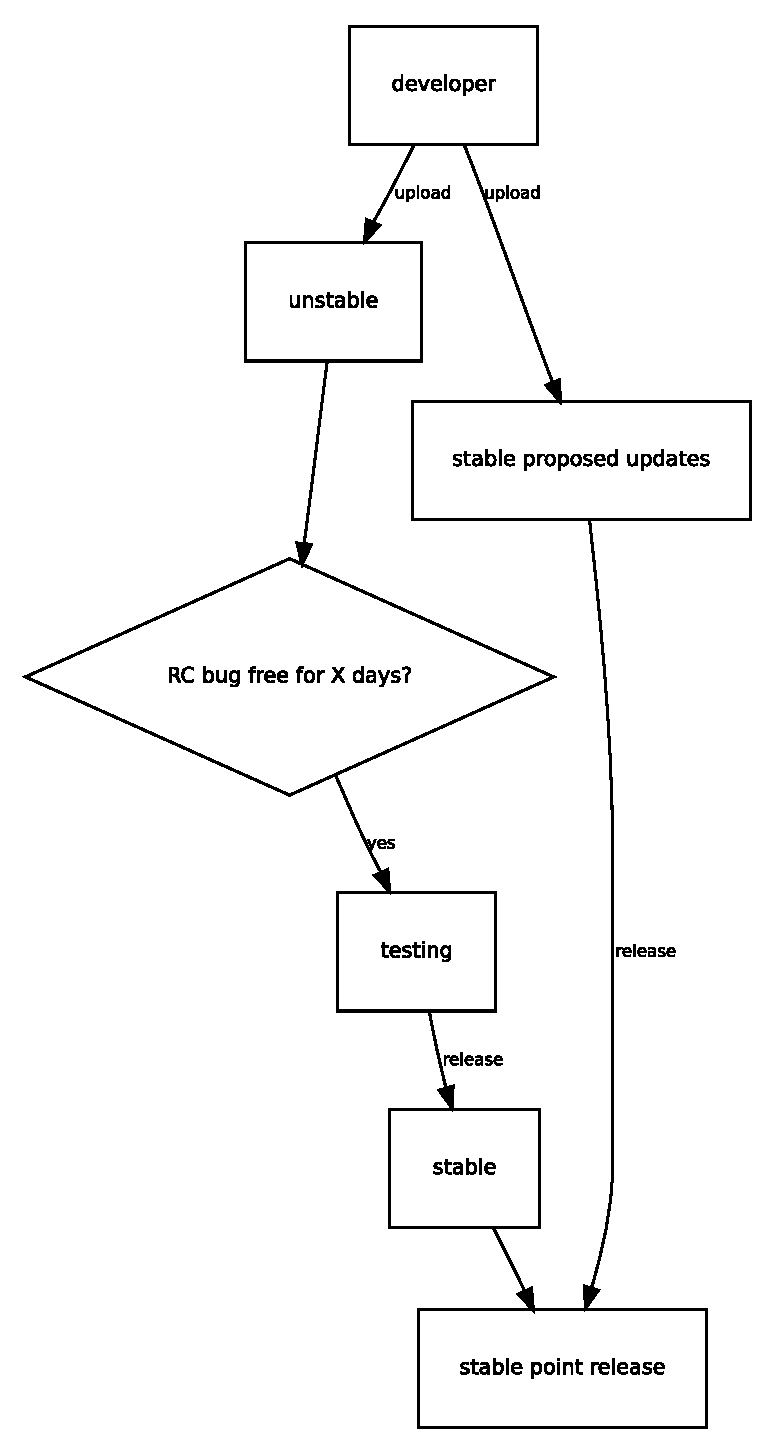
\includegraphics[width=1\hsize]{image200805/testingcycle.eps}
\end{minipage}
\end{frame}

\begin{frame}{Developer Process: bug receive}
 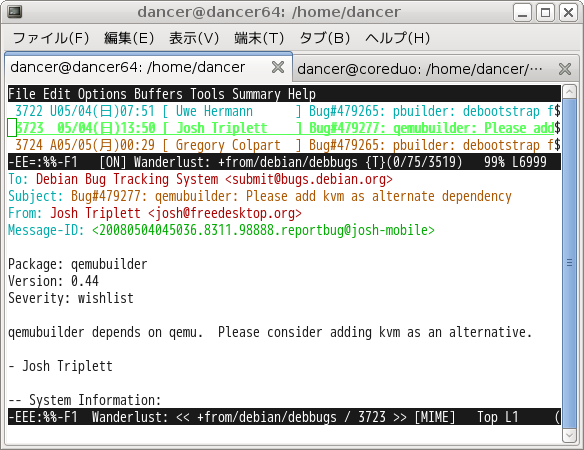
\includegraphics[width=1\hsize]{image200805/bug1.png}
\end{frame}

\begin{frame}{Developer Process: bug analyse}

....
\end{frame}

\begin{frame}{Developer Process: bug fix 1/3}
 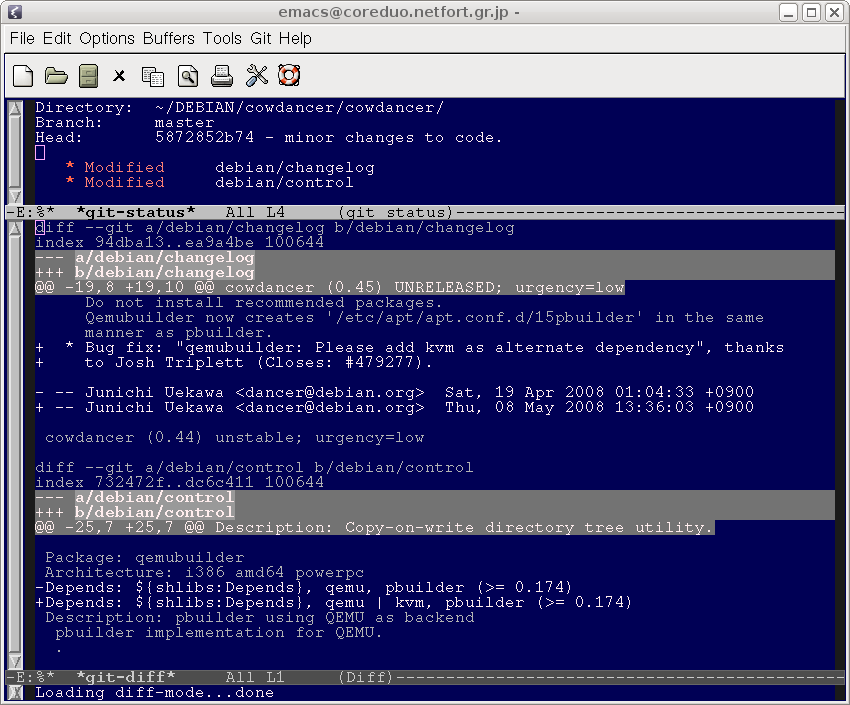
\includegraphics[width=1\hsize]{image200805/bug2.png}
\end{frame}

\begin{frame}[containsverbatim]{Developer Process: bug fix 2/3}

bug is closed on changelog entry.

\begin{commandline}
cowdancer (0.45) unstable; urgency=low

  * cowbuilder, qemubuilder: Give error message when '--build' is invoked
    without .dsc file parameter.  (Closes: #460041).
  * output more useful info on waitpid WIFEXITED debug message.
  * add header to .ilist, so that it is possible to know a little bit more
    about the structure.  Note that upgrade will fail within cowdancer
    session, please re-create chroot, or use the --no-cowdancer-update option:

      Unpacking cowdancer (from .../cowdancer_0.45_amd64.deb) ...
      ERROR: ld.so: object '/usr/lib/cowdancer/libcowdancer.so' from LD_PRELOAD cannot be preloaded: ignored.
      cowdancer: .ilist header unexpected
      cowdancer: .ilist header unexpected
      cowdancer: .ilist header unexpected
      dpkg-split: unable to read part file `/tmp/buildd/qemubuilder_0.45_amd64.deb': Cannot allocate memory
      dpkg: error processing /tmp/buildd/qemubuilder_0.45_amd64.deb (--install):
  * Bug fix: "qemubuilder --create installs many useless? packages",
    thanks to David Bremner (Closes: #476547).
    Do not install recommended packages. 
    Qemubuilder now creates '/etc/apt/apt.conf.d/15pbuilder' in the same
    manner as pbuilder.
  * Bug fix: "qemubuilder: Please add kvm as alternate dependency", thanks
    to Josh Triplett (Closes: #479277).

 -- Junichi Uekawa <dancer@debian.org>  Thu, 08 May 2008 13:36:03 +0900
\end{commandline}
\end{frame}

\begin{frame}{Developer Process: bug fix 3/3}
 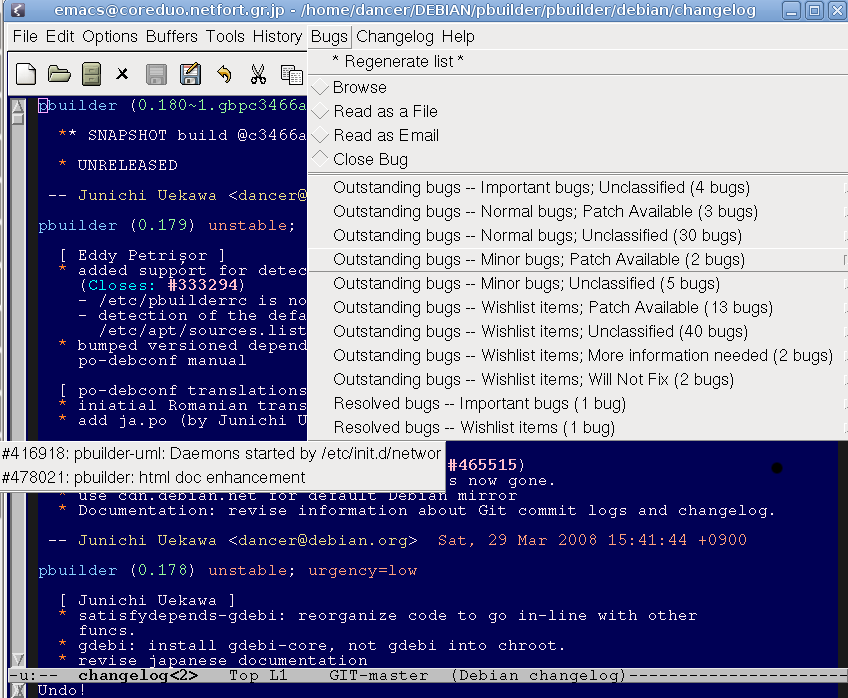
\includegraphics[width=1\hsize]{image200805/bugclosing.png}
\end{frame}

\begin{frame}{Developer Process: package upload}
\begin{itemize}
 \item debuild: build package
 \item pdebuild / cowbuilder: build in clean-room environment
 \item debi / dpkg -i: install locally (for testing)
 \item debsign: GPG-sign (cryptographically sign for authentication)
 \item dput / dupload: release to 'unstable' users
\end{itemize}
\end{frame}

\begin{frame}{Debian Development Process}

 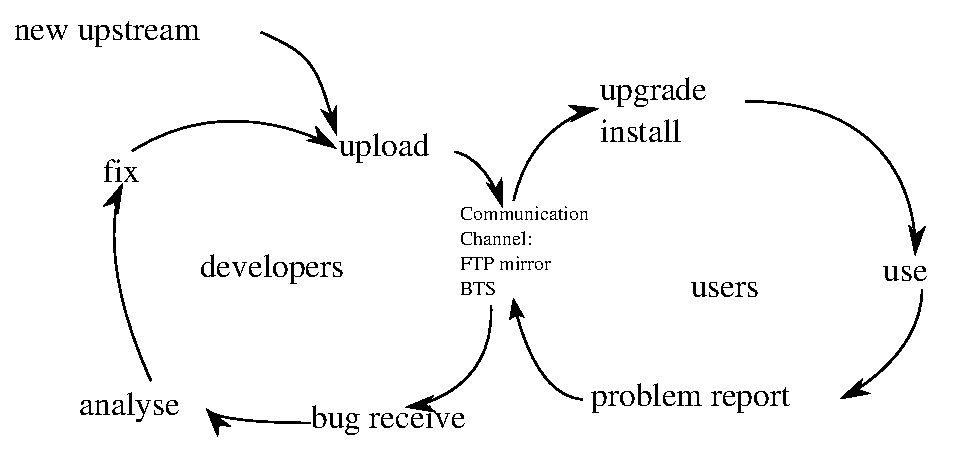
\includegraphics[width=1\hsize]{image200805/develcycle.eps} 

\end{frame}

\begin{frame}{localization}
 There are different localization aspects. Looking at translation at
 random gives:
\begin{itemize}
 \item po: upstream translation, shared with other distributions etc.
 \item po-debconf: debconf prompt translation.
 \item debian.org, webwml: web page translation
 \item DDTP/DDTSS: Description translation
 \item po4a: tool to support translation
 \item i18n task force: \url{http://i18n.debian.net}
\end{itemize}
\end{frame}

\begin{frame}{localization: po editors}

    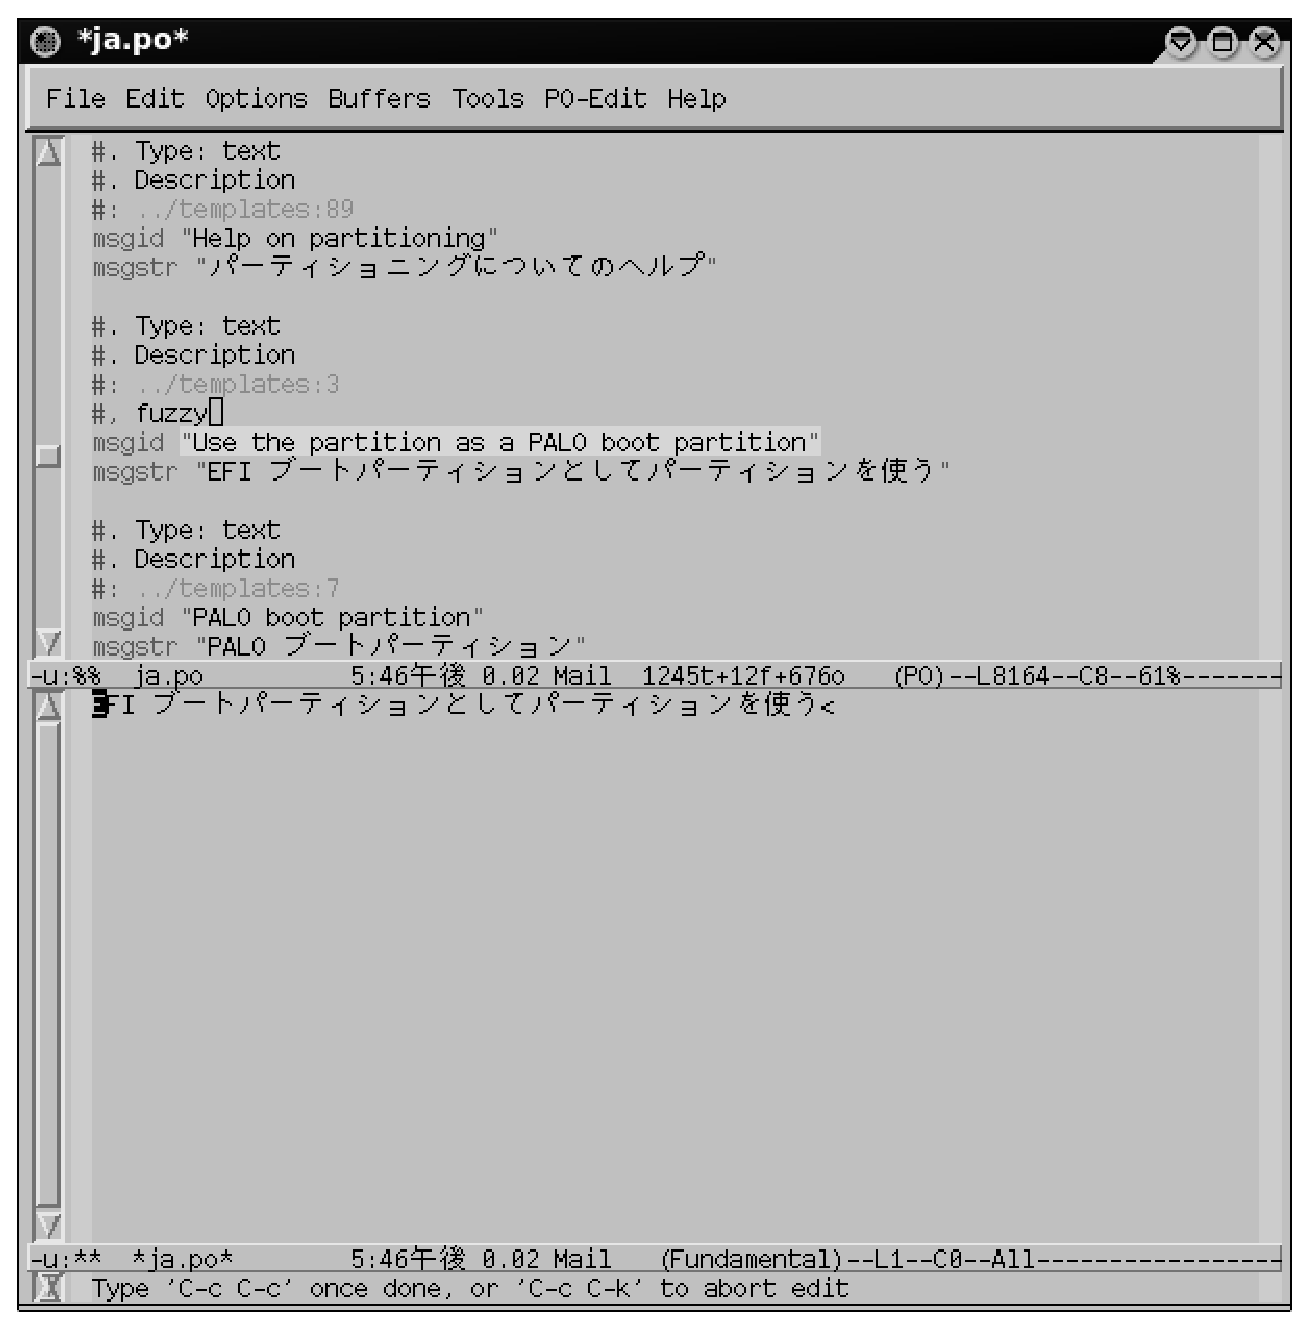
\includegraphics[width=0.4\hsize]{../2006-resume/image200610/emacs-po.eps}
    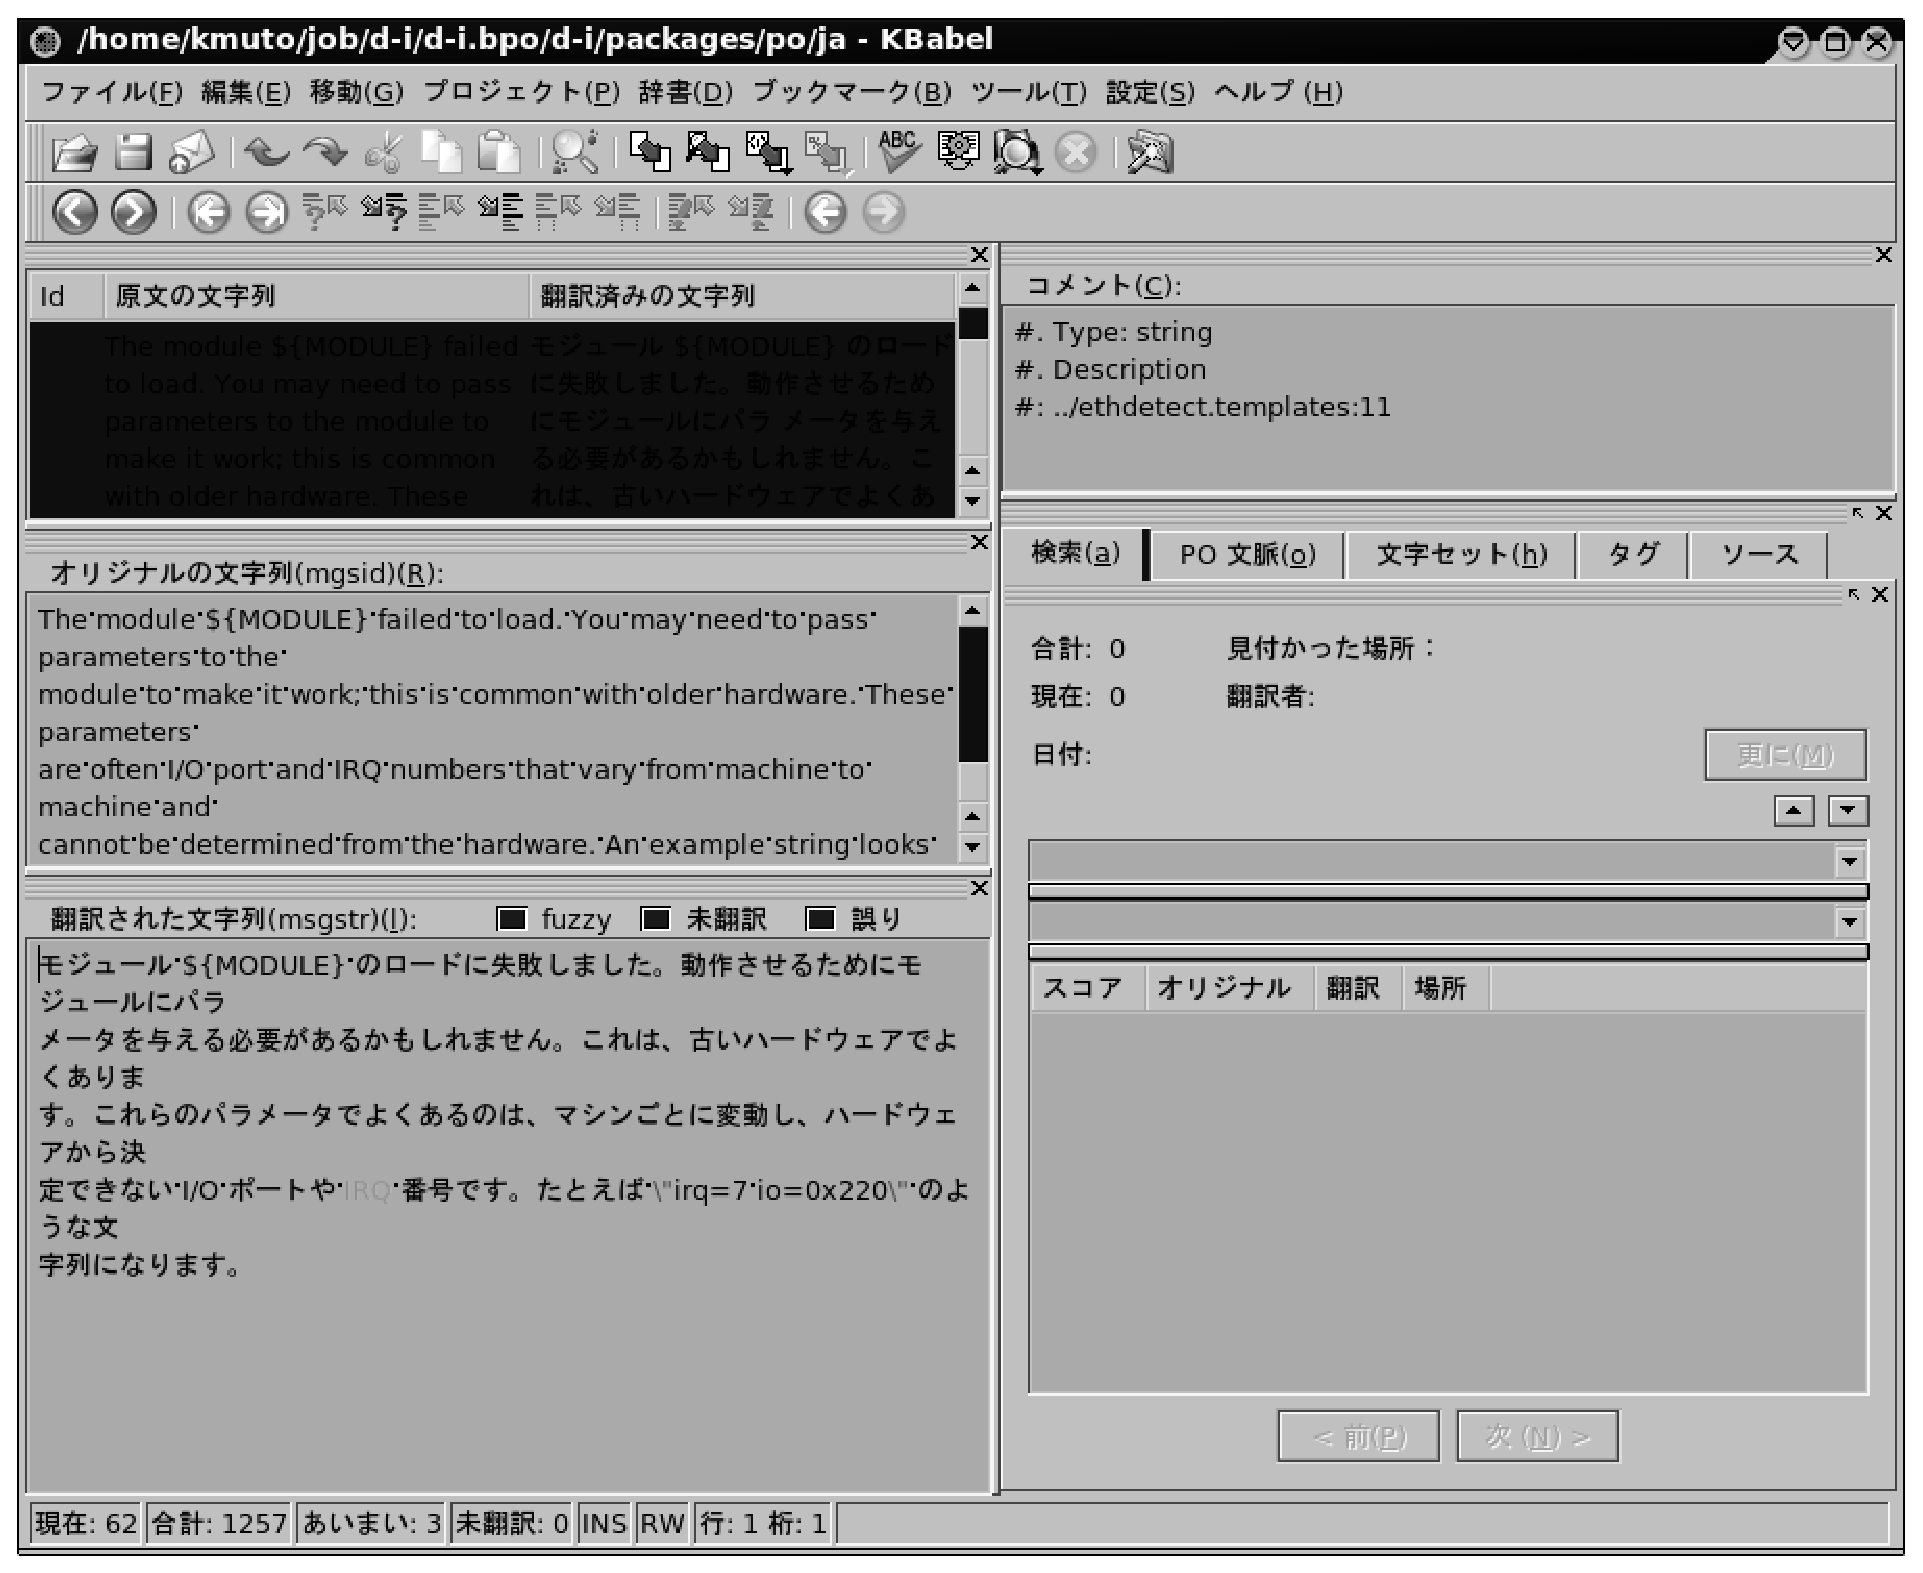
\includegraphics[width=0.4\hsize]{../2006-resume/image200610/kbabel.eps}

    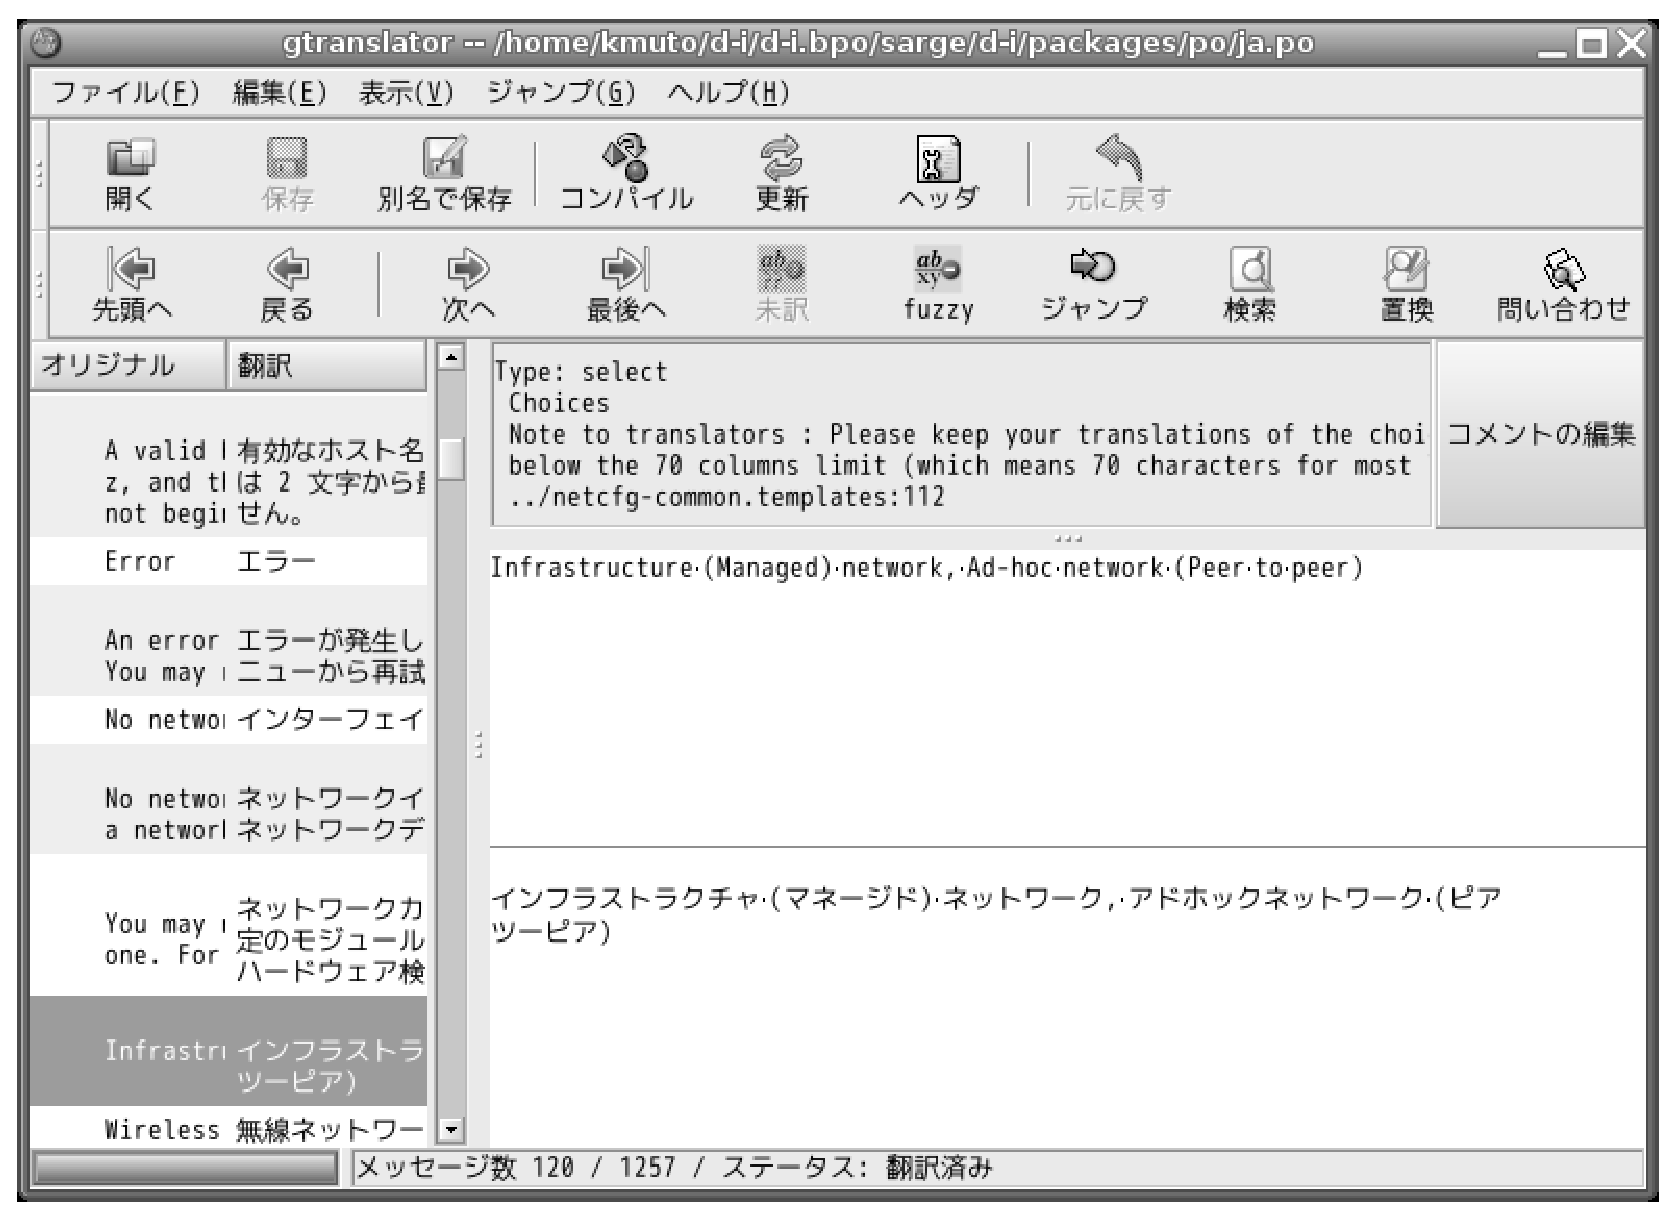
\includegraphics[width=0.4\hsize]{../2006-resume/image200610/gtranslator.eps}
\end{frame}

\begin{frame}{localization: po-debconf}

 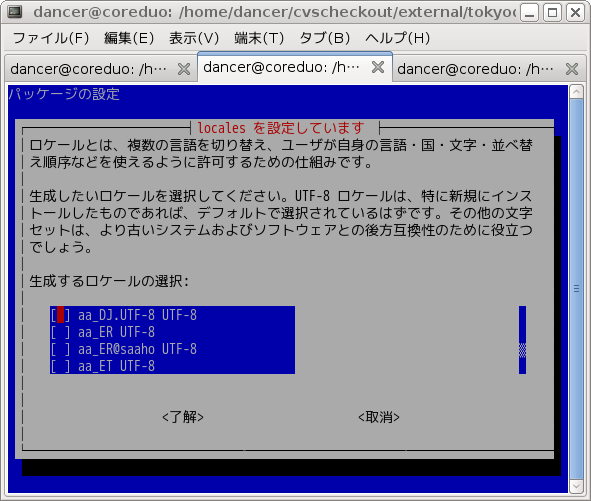
\includegraphics[width=0.5\hsize]{image200805/debconf-text.png}
 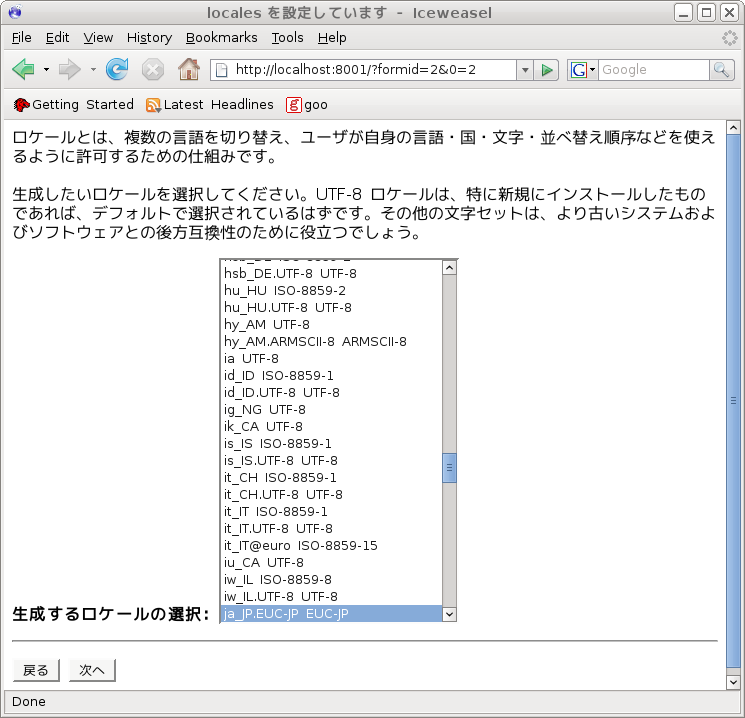
\includegraphics[width=0.5\hsize]{image200805/debconf-locales.png}

\end{frame}

\begin{frame}{i18n task force}
 \begin{itemize}
  \item i18n task force: \url{http://i18n.debian.net}
  \item IRC channel \url{\#debian-i18n@irc.debian.org}
 \end{itemize}
\end{frame}

\begin{frame}{Case study: Debian eeePC project}
 \begin{itemize}
  \item Porting Debian to eeePC as CDD
  \item Try to provide extra packages and integrate patches
  \item \url{http://wiki.debian.org/DebianEeePC}
  \item Mailing list: \url{http://alioth.debian.org/mail/?group_id=31309}
  \item IRC channel: \url{irc://irc.oftc.net/\#debian-eeepc}
 \end{itemize}
\end{frame}

\begin{frame}{What's Next}
 \begin{itemize}
  \item Taipei Debian Community Kick off 
	-- Be part of the next movement
  \item 10 May 2008 (Sat)
 \end{itemize}
\end{frame}


\end{document}

;;; Local Variables: ***
;;; outline-regexp: "\\([ 	]*\\\\\\(documentstyle\\|documentclass\\|emtext\\|section\\|begin{frame}\\)\\*?[ 	]*[[{]\\|[]+\\)" ***
;;; End: ***
